\subsection{TorCoin Mining}

Mining TorCoin requires transferring bandwidth. We introduce a novel method to
prove end-to-end bandwidth transfer across a Tor circuit.

\begin{figure}[H]
  \centering
    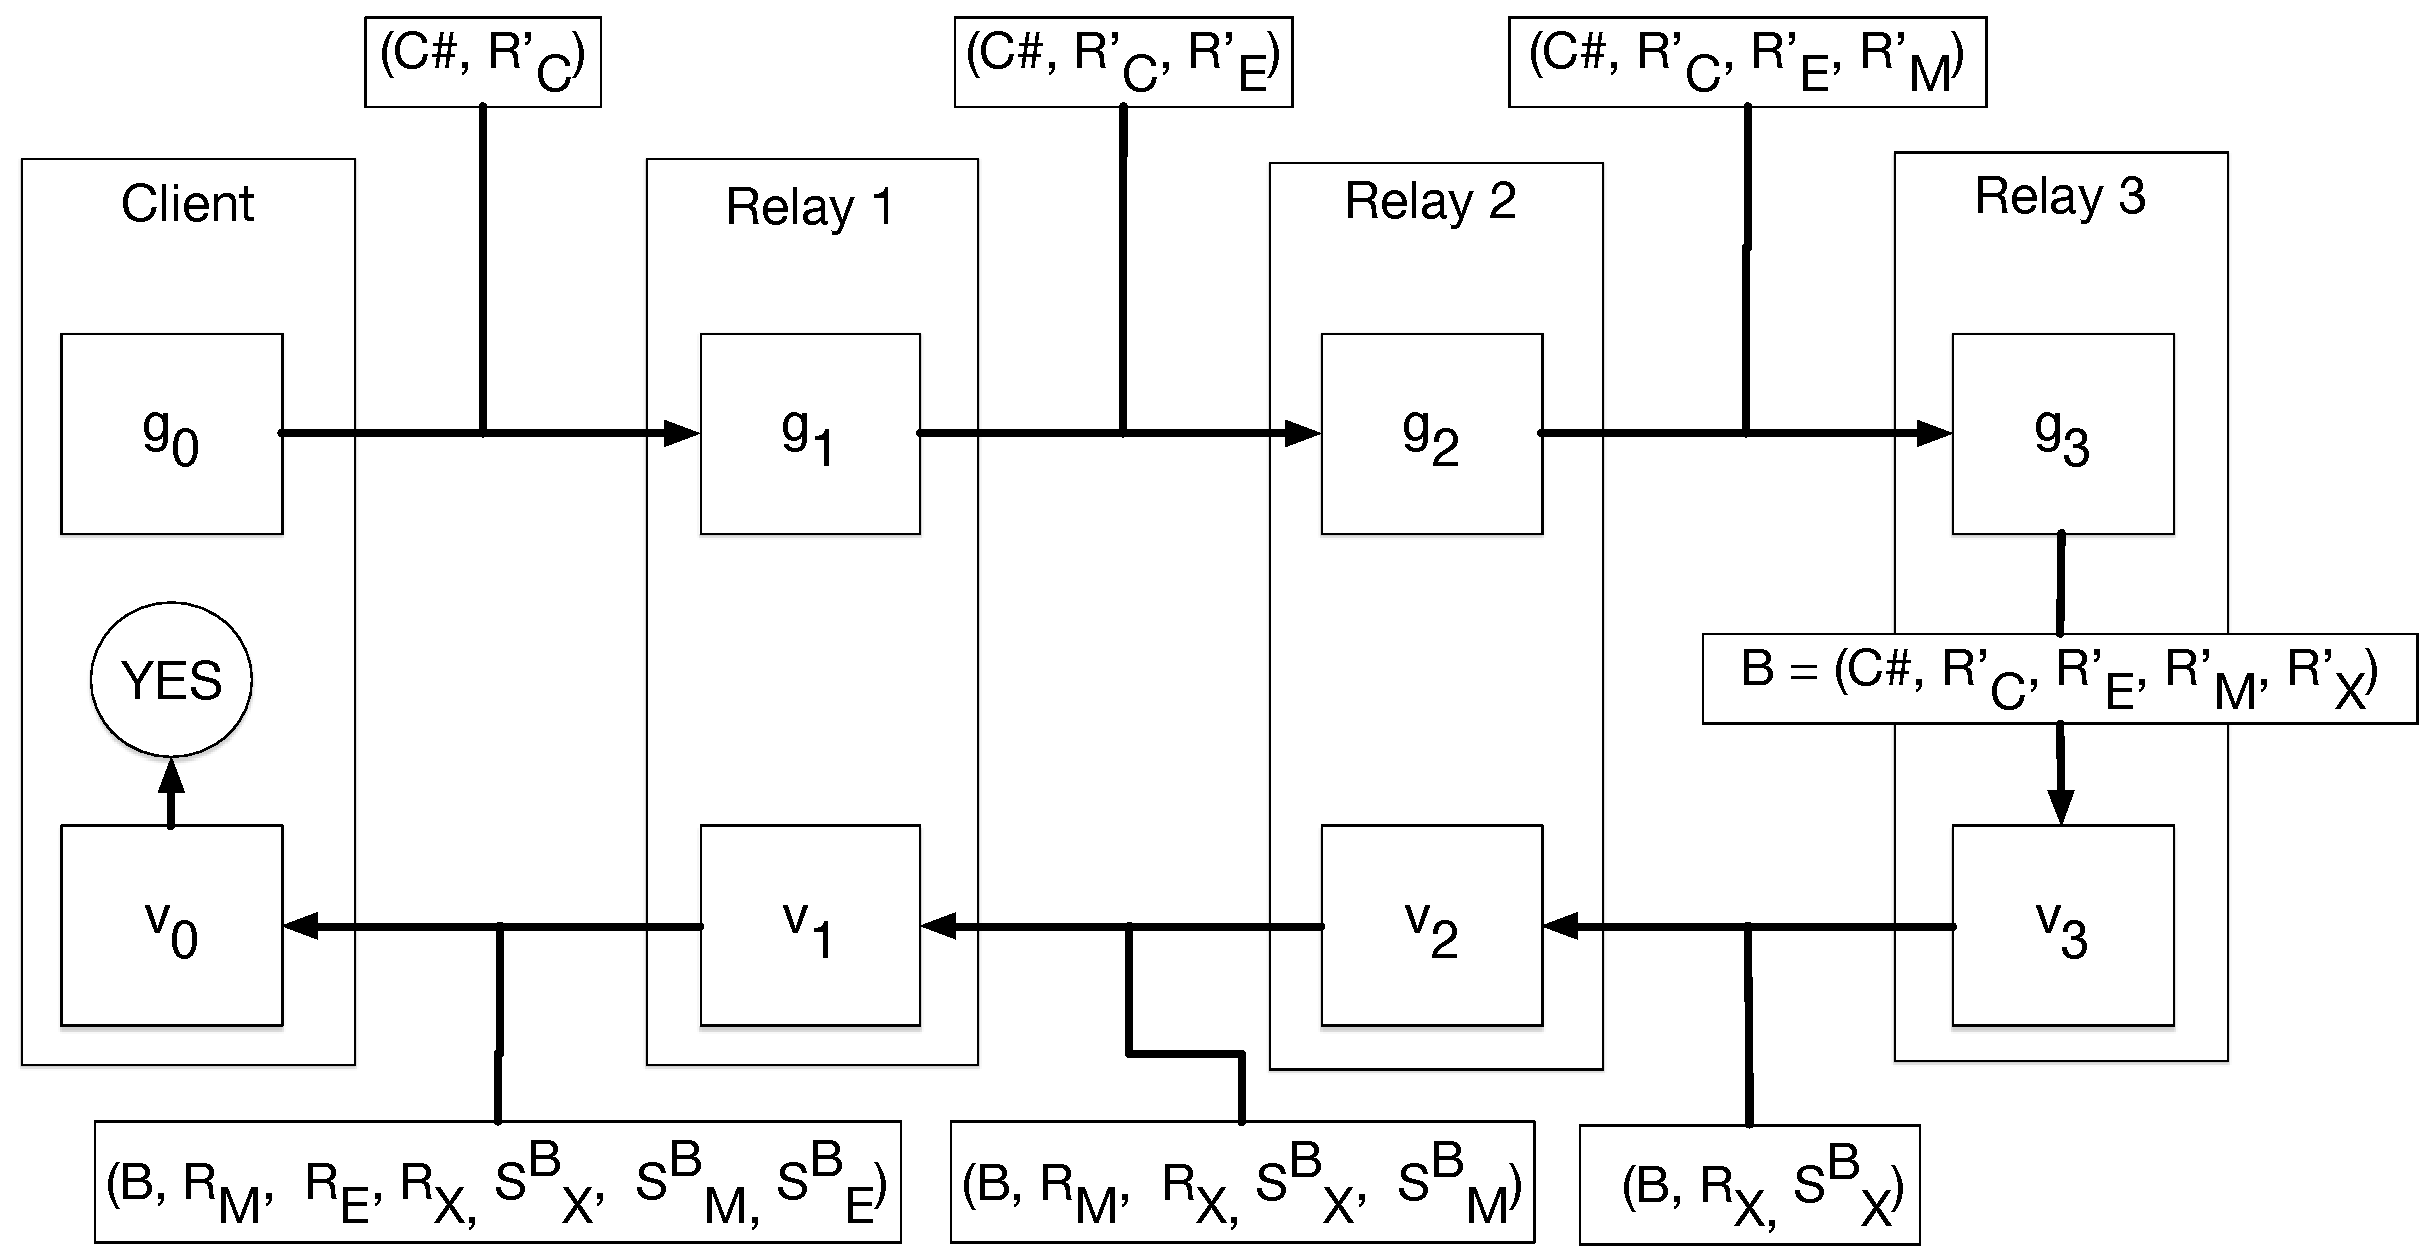
\includegraphics[scale=0.3]{torcoin_cycle.pdf}
  \caption{TorCoin Proof of Bandwidth algorithm. In the upper part of the cycle, the relays add their hashes to the tuple. In the lower part, they add their temporary keys and sign the tuples.}
\end{figure}

\subsubsection{Proof of Bandwidth}
\begin{enumerate}
\item Each client and relay creates a temporary key R and its hash $R_*' = Hash(R_*)$. 
\item Every $m$ Tor packets, the client sends a tuple (coin\#, $R'_C$), where coin\# is the number of Tor packets sent in this circuit.
\item Each relay adds its own temporary hash to the tuple and sends it to the next relay in the circuit.
\item The exit relay adds its own hash to the tuple to create the coin blob 
$B = (coin\#, R'_{C}, R'_{E}, R'_{M}, R'_{X})$ 
\item The exit relay then signs the blob B to create $S^B_X$ and sends the tuple $(B, S^B_X, R_X)$ to the middle relay.
\item Each of the relays, $i$, signs the blob B to create $S^B_i$ and adds their signature and their temporary key to the tuple, and forwards it to the previous component in the circuit. 
\item The client receives the tuple $candidate = (B, S^B_X, S^B_M, S^B_E, R_X, R_M, R_E, R_C)$ and verifies its correctness, thus proving bandwidth transfer.
\item To check if a TorCoin has been minted, the client checks if the lower-order bits of $Hash(CS_i, candidate) == 0$. If so, the client adds the tuple $(CS_i, candidate)$ to the blockchain to mint a ``TorCoin''.
\item The client then pays each relay in the circuit $\frac{1}{3}$ of the TorCoin. 
\end{enumerate}

All the information necessary for verifying proof-of-bandwidth is in the
blockchain. Any interested party can then verify that the route signature is
authentic and refers to the correct group by referring to the public log. They
can also verify that the blob B was signed by the correct relays by verifying
the signatures, as well as verify that the temporary keys R actually hash to
the claimed values R'.

\subsubsection{Security Considerations}

\paragraph{Enforcing packet rate} All honest relays and clients
enforce the TorCoin packet rate $m$. Any relays or clients that deviate from this
are reported to the assignment servers and the circuit is terminated.

\paragraph{Enforcement of TorPath circuits} Relays know their neighbours'
IP addresses and will refuse connections from any other IP address. Even if
malicious relays connect to each other, they will not be able to sign each
other's TorCoins since they do not have the circuit signature.

\paragraph{Compromised circuits} Any system of colluding clients and
attackers needs to control all four components of a route to mint a TorCoin
fraudulently. Even if an adversary controls up to half the network, there is a
probability of only $(\frac{1}{2})^4 = \frac{1}{16}$ that an adversary client
gets a path of three colluding relays. In practice, gaining control of half of
all Tor clients and relays would be hard for an adversary.  To limit the
impact of these malicious circuits, the network imposes a limit on the number
of coins that can be mined by a particular circuit. This coin number is
included in the blockchain, so it is easily verified. 
The impact of these
compromised circuits can be further reduced by ensuring that consensus groups
expire at frequent intervals, requiring clients to change their circuits.

\subsubsection{Drawbacks} The TorPath network is not backwards compatible with
the existing Tor network, due to the fundamental differences of route
assignment and access control, which are missing in Tor, but are necessary for
the TorPath and TorCoin schemes to work.

However, our scheme does not preclude a given physical relay or server from
running both services at the same time. They will, of course, only get paid
for the TorCoin traffic. In time, we expect that a majority of the current Tor
relay operators will switch over to the TorPath network, since TorPath has the
same security guarantees as Tor provides, while also recompensing the relay
operators for their costs.

Backwards-compatible Tor incentivization schemes like LIRA have significant
drawbacks like the usage of Eigenspeed for bandwidth measurement or the
establishment of a central bank to keep track of their tokens. These all
introduce significant infrastructure into the Tor network and may reduce
anonymity.
